%!TEX TS-program = pdflatex 

\documentclass[10pt,usletter]{article}
\usepackage{url}
\usepackage[table,x11names,svgnames]{xcolor}
\usepackage[francais]{babel}
\usepackage{fancybox, paralist}
\usepackage{titlesec}
\usepackage{pdfpages}
\usepackage{hyperref}
\hypersetup{ 
     colorlinks=true,
     breaklinks=true,
     urlcolor= blue,
     linkcolor= Blue3,
     citecolor=Green,
     bookmarksopen=true
}
\usepackage{tcolorbox}

\usepackage[utf8]{inputenc}
\usepackage{fourier}
%\usepackage{antpolt}
\usepackage[T1]{fontenc}

\textwidth = 6.5 in
\textheight = 9 in
\oddsidemargin = 0.0 in
\evensidemargin = 0.0 in
\topmargin = -0.25 in
\headheight = 14pt
\headsep = 0.2 in
\parskip = 0.1in
\parindent = 0.0in
\def\bigstrut#1{\vrule height #1 ex width 0pt depth 4pt}

\titleformat{\section}{\penalty-2000\vspace{0pt plus 10pt}{\color{DodgerBlue4!80!black}\titlerule[2pt]}\large\bfseries\sffamily}{\thesection}{1em}{}[\vspace{2pt plus 2pt}{\color{DodgerBlue4!80!black}\titlerule[1pt]}] 

\titleformat{\subsection}[runin]{\bfseries\sffamily}{\thesubsection}{}{}[.~~]

\tcbuselibrary{raster}
\tcbset{tcbplanstyle/.style={
	coltitle=black, 
	coltext=black, 
	colframe=gray!20!white, 
	colback=white,
	leftrule=1pt, 
	rightrule=1pt, 
	toprule=1pt, 
	bottomrule=1pt,
	arc = 0.5mm,
	left =2mm, 
	right =2mm,
	fonttitle=\bfseries
}}

%---------------------------------------------------------------------------
\begin{document}

\parbox{5cm}{\includegraphics[scale=0.45]{UdeS_physique}}
\hfill\parbox{3cm}{\raggedleft Plan de cours\\
Hiver 2023\\
~~
}

\begin{center}
{\Large\textcolor{DarkRed}{INTRODUCTION~~AU~~CALCUL~~SCIENTIFIQUE}}\\
\href{http://www.usherbrooke.ca/moodle2-cours/my}{www.usherbrooke.ca/moodle2-cours/my}
\bigskip


\begin{tcbraster}[raster columns=2, 
	raster valign=top, 
	raster left skip=0mm, 
	raster right skip=0mm,
	raster column skip=2mm
]
%
\begin{tcolorbox}[tcbplanstyle, title = Cours]
Titre: ~ Introduction au calcul scientifique\\
Sigle: ~ PHQ202\\
Crédits: ~ 2\\
Travail personnel: $\sim$ 45 heures au total.
\end{tcolorbox}
%
\begin{tcolorbox}[tcbplanstyle, title = Professeur]
Nom:~ David Sénéchal\\
Bureau:~ D2-1068\\
Tél.:~ 821-8000 poste 62053\\
Courriel:~ david.senechal@usherbrooke.ca
\end{tcolorbox}
%
\begin{tcolorbox}[tcbplanstyle, title = Place du cours dans le programme]
Type de cours:~ obligatoire\\
Cours préalables:~ aucun\\
Cours concomitants:~ IFT211
\end{tcolorbox}
%
\begin{tcolorbox}[tcbplanstyle, title = Moniteur/correcteur]
Nom:~ Céline Zhang\\
% Bureau:~ ***\\
Courriel:~ celine.zhang@usherbrooke.ca
\end{tcolorbox}
%
\end{tcbraster}
\end{center}

%---------------------------------------------------------------------------
\section{Objectifs}

\subsection*{Objectif général}
Résoudre des problèmes numériques de la physique à l'aide d'un langage de haut niveau.

\subsection*{Sommaire des thèmes}
\begin{compactenum}[~~1.~]
\parskip = 0.0in
\item Bibliothèques scientifiques en Python: NumPy, SciPy, Matplotlib
\item Modélisation de données
\item Matrices et algèbre linéaire
\item Applications à la mécanique : équations différentielles
\item Applications à l'électromagnétisme
\item Applications aux phénomènes ondulatoires
\item Simulation des populations
\item Outils divers : Sympy, UNIX, etc
\end{compactenum}

%----------------------------------------------------------------------------
\section{Méthode pédagogique}

\begin{compactenum}[1.~]
\item Chaque semaine de cours est associée à un thème précis.
\item Chaque semaine l'étudiant(e) devra lire un matériel préalable ou visionner une vidéo tenant lieu de cours magistral. La première heure du vendredi sera consacrée à répondre aux questions ou a discuter du matériel. La méthode s'inspirera de l'enseignement inversé.
\item L'heure suivante à l'horaire sera consacrée à des exercices obligatoires portant sur la matière de la semaine courante, avec une remise individuelle d'un bloc-note python à la fin de l'heure. Il ne s'agit pas d'un travail d'équipe. Le professeur sera présent pour répondre aux questions individuelles.
\item Deux heures/sem. (les mardis) seront consacrées aux travaux pratiques, qui seront effectués en équipes de deux et remis au début de la semaine suivante. La monitrice (Mme Céline Zhang) sera sur place lors de cette période. Notez que les travaux pratiques seront initiés à chaque semaine (mardi) avant la période de questions et d'exercices (vendredi).
\end{compactenum}

Le seul logiciel requis est un navigateur afin d'accéder au serveur jupyter du cours.

%---------------------------------------------------------------------------
\section{Évaluation}

\begin{compactenum}[1.~]
\item Sept devoirs (ou TP), pour 50\% de la note finale. Les devoirs devront être remis par équipes de deux ou, exceptionnellement, individuellement, sous la forme de bloc-notes Python (fichiers .ipynb) comportant des \textit{explications} et du \textit{code}. La remise des travaux se fera sur Moodle. Les noms des deux membres de l'équipe doivent clairement figurer en haut du bloc-note. Les équipes peuvent changer d'un TP à l'autre et ne sont pas assignées par le responsable du cours.
\item Les exercices hebdomadaires faits en classe, pour 50\% de la note finale. Ils doivent être remis sur une base individuelle (ce n'est pas un travail d'équipe). Les exercices seront disponibles au début de l'heure sur le serveur jupyter et pourront être remis (la procédure sera expliquée en classe) pendant l'heure qui suit. Il est \textbf{très important} de bien lire le matériel préalable pour être en mesure de faire les TP et de bien solutionner les exercices dans le temps alloué.
\item En tout temps l'étudiant(e) a accès au réseau et aux ressources disponibles sur le web.
\end{compactenum}
Le calendrier des thèmes et des travaux est en annexe.

%---------------------------------------------------------------------------
\section{Matériel pédagogique}

Les étudiants ont accès à un serveur {\it Jupyter Lab}:

\href{https://phy-jpthub.ccs.usherbrooke.ca}{https://phy-jpthub.ccs.usherbrooke.ca}

Le code d'accès est le CIP de l'UdeS. Le mot de passe initial sera décrit lors du premier cours.
Le mot de passe peut être modifié en utilisant la commande \texttt{passwd} sur un terminal qui peut être ouvert au sein même d'une session {\it Jupyter Lab}.

Ce serveur contient un répertoire public (/home/dsenech/public) contenant les fichiers pertinents au cours, en particulier le matériel à étudier pour chaque thème. Le matériel principal consiste en bloc-notes ({\it notebooks}) Python et en notes diverses en format PDF.
Aucun autre matériel n'est obligatoire.

Des \textbf{vidéos} sont disponibles sur youtube:

\url{https://www.youtube.com/watch?v=VQuAdSva0Tc&list=PLzniPINhDCMMhf9xgoA1ajoADCGf-Sz7O}

 Ces vidéos font office de cours magistraux et \textbf{doivent être visionnés avant la période du mardi} assignée à chaque thème. 

\begin{center}
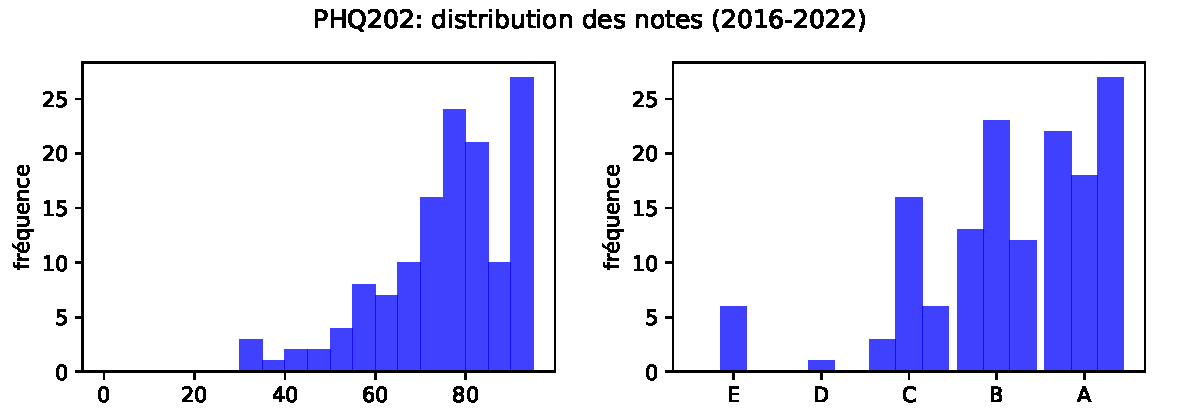
\includegraphics[width=\hsize]{stats.pdf}
\end{center}

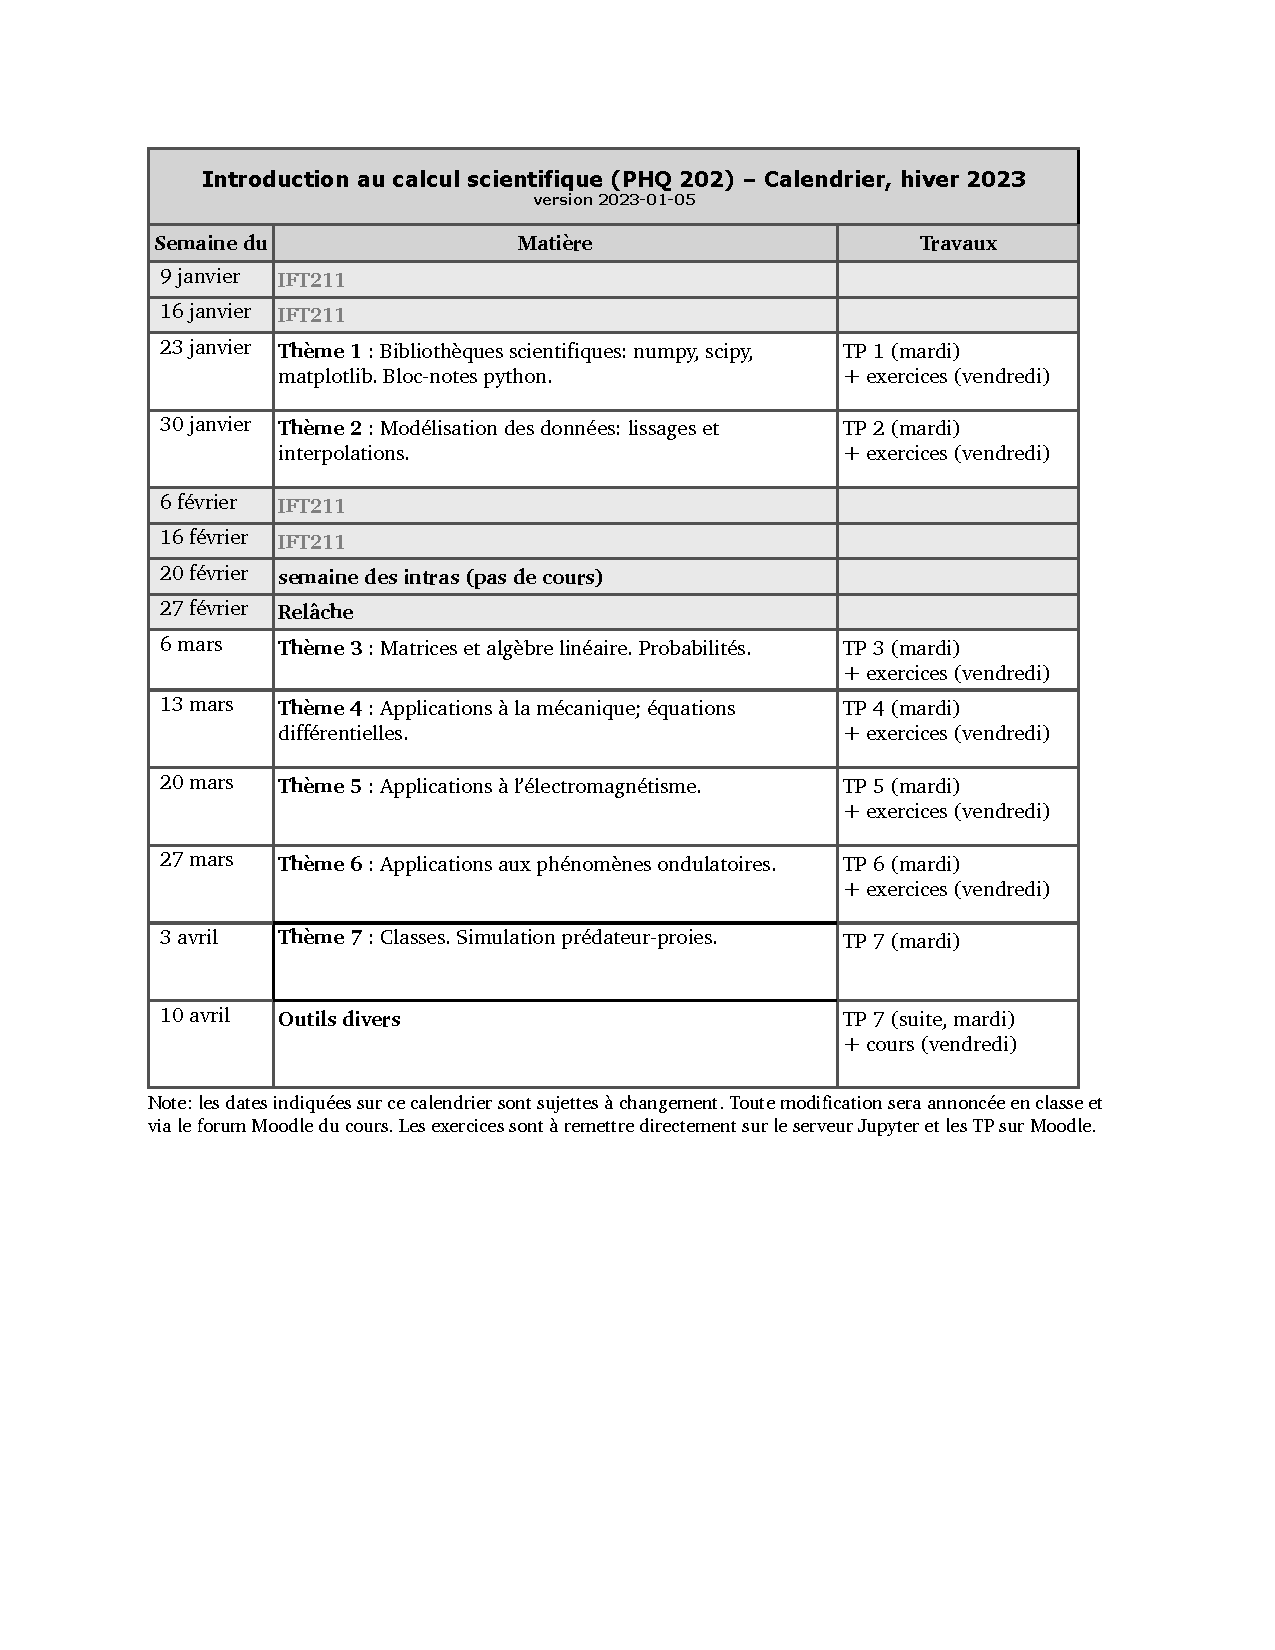
\includepdf[pages=-]{PHQ202-calendrier-2023}
\end{document}

